\bigskip
\begin{center}\textsc{Gauss} to \textsc{Gerling}.\quad Göttingen, 5 June 1838.\end{center}

According to a theorem that I am unsure whether I have communicated to you before,
if $p$ points in a system of triangles are connected by $l$ lines, whether
the directions of those lines are fixed in only one direction or in both
directions, one must obtain, in addition to the condi-\par
\makeatletter
\def\ps@gaussIXfortyonestar{\def\@oddhead{}\def\@evenhead{}\def\@oddfoot{\hfil41\textsuperscript{*}\hspace{2em}}\let\@evenfoot\@oddfoot}
\makeatother
\thispagestyle{gaussIXfortyonestar}
\clearpage
\noindent324\hfill\textbf{CORRESPONDENCE.}\par\medskip
\noindent tion equations of the (first and) second classes [the horizon closures
and the angle equations], a further $l-2p+3$ mutually independent condition
equations. \textls[120]{Neither more nor fewer.} It may happen that they cannot all
be put in the form of the third class [the side equations], for example in
a ring of triangles.
\begin{center}
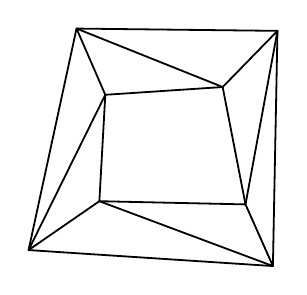
\begin{tikzpicture}[x=.58cm,y=.58cm,line width=.65pt,line cap=round,line join=round]
\coordinate (A) at (1.05,5.3);
\coordinate (B) at (5.45,5.25);
\coordinate (C) at (5.35,0.1);
\coordinate (D) at (0,0.45);
\coordinate (E) at (1.68,3.85);
\coordinate (F) at (4.25,4.02);
\coordinate (G) at (4.75,1.45);
\coordinate (H) at (1.55,1.52);
\draw (A)--(B)--(C)--(D)--cycle;
\draw (E)--(F)--(G)--(H)--cycle;
\draw (A)--(E) (A)--(F) (B)--(F) (B)--(G)
      (C)--(G) (C)--(H) (D)--(H) (D)--(E);
\end{tikzpicture}
\end{center}

I leave this exception aside, however, as it need not be considered in your
system.

I now count
\[
\begin{aligned}
p&=24\ \text{points}\\
l&=66,\ \text{namely }\begin{aligned}[t]22\ &\text{one-way directions,}\\44\ &\text{reciprocal directions,}\end{aligned}
\end{aligned}
\]
so that there must be 21 condition equations of the kind in question, and
that is indeed how many you have. One can test their independence by
ordering the $p$ points suitably, in doing which I had to depart in part from the
order of your numbers 1 .\ .\ .\ .\ 112, and applying the same theorem
repeatedly as one brings in the $p$ points in succession until all are
included. Your 21 equations passed this test as well. There is some
confusion in \textls[120]{your} numbering; 24 and 61 are missing, so that there
are in all (as above $22+2\mathbin{.}44)=110$ directions, and 112 is in the wrong place.

After this test I have no doubt that you can present your 21 equations
without hesitation.

If I have counted correctly, you must also have 24 condition equations of
the $2^{\mathrm{nd}}$ class.

I must call your attention to one point about carrying out the work. If I
have already done so, let the good intention excuse my forgetfulness.

In setting out your tables you depart from my form in that you reckon all
directions from \textls[120]{one of them}, whereas I reckon from a direction that
is to some extent arbitrary, or, more accurately,\par
\clearpage
\noindent\textbf{ON NETWORK ADJUSTMENT.}\hfill325\par\medskip
\noindent external to the system. You must therefore remember when carrying out the
work that all directions are equally reliable, or, more accurately, equally
unreliable, so that you must include your 0 each time among the directions
requiring correction. In every case the result will be that the sum of all
corrections at a single station becomes $=0$.

\begingroup
\def\letterfivestars{*}
\makeatletter
\renewcommand{\@makefnmark}{\hbox{\normalfont[\textsuperscript{\letterfivestars})]}}
\renewcommand{\@makefntext}[1]{\parindent1em\noindent\hbox to2.4em{\hss[\textsuperscript{\letterfivestars})\ }#1]}
\makeatother
But I admire your intrepidity in taking on so great a task of elimination.
I would not have had the same courage. For my 33 points the number of
condition equations of the $3^{\mathrm{rd}}$ class [the side equations] was
much smaller (7, I believe)\footnote{There are 12.}. When one took into account
at first only the equations of the $2^{\mathrm{nd}}$ class [the angle equations],
elimination by an indirect method was easy despite the large number of these
equations, and errors in the calculation were impossible. The fact that all directions
had been measured both ways allowed modifications that greatly eased the
work and let me reach stable results quickly. I fear the latter will hold
to a much lesser degree in your case\def\letterfivestars{**}\footnote{See pp.\ 250/251.}.
But once you have set yourself the objective, the only means are attention
and patience.

Had I had to carry out these calculations myself, I would have left the
three places at which no measurements were made entirely out of the system,
not because I disapprove of including them, but because I would have
shied away from the great amount of work. If all directions observed from
only one end were excluded, the adjustment of the system would be
very easy, but to be sure, in your undertaking taking them fully into
account adds considerably to the reliability. .\ .\ .\ .\ .\ .

The arrangement for the quadrilaterals is in itself arbitrary, and it is
only to eliminate that arbitrariness that I follow the rule you
cited\def\letterfivestars{***}\footnote{See the letter to \textsc{Gerling} of 11 February 1824, p.\ 249. With reference to it,
\textsc{Gerling} had written (on 2 June 1838): “So far I have been able to give myself no other account of the reason
for the rule than that in this way the comparatively largest coefficients appear.”}, which has no advantage beyond the one you correctly surmised.
\endgroup
